\documentclass{beamer}

\usetheme{CambridgeUS}

\usepackage{fourier}

\usefonttheme{professionalfonts} % using non standard fonts for beamer
\usefonttheme{serif} % default family is serif
\usepackage{fontspec}
\setmainfont{ClearSans-Regular.ttf}

\usepackage{tcolorbox}
\usepackage{lipsum}

\usepackage{algorithm}
\usepackage{algpseudocode}
\makeatletter
%\algrenewcommand\ALG@beginalgorithmic{\tiny}
\makeatother

% NEW COMMENTS
\newcommand{\MO}{\mathcal{O}}


% SECTION TITLE SLIDE

\AtBeginSection[]{
	\begin{frame}[plain]
	\vfill
	
	\centering
	\begin{beamercolorbox}[center,rounded=true]{body}
		\usebeamerfont{title}\insertsectionhead\par%
	\end{beamercolorbox}
	\rule{20pt}{1pt}
	\vfill
\end{frame}
}


% COLOR
\definecolor{C}{HTML}{20639b}
\definecolor{CL}{HTML}{FCB76F}
\definecolor{CD}{HTML}{541D61}
\definecolor{GrD}{HTML}{8F3066}
\definecolor{GrL}{HTML}{EEEEEE}

\definecolor{W}{HTML}{FFFFFF}

\setbeamercolor{palette primary}{fg = W,bg = CD}
\setbeamercolor{palette secondary}{fg = CL,bg = CD}
\setbeamercolor{palette tertiary}{fg = CL,bg = CD}
\setbeamercolor{palette quaternary}{fg = CL,bg = CD}

\setbeamercolor{title}{fg = CL,bg = CD}
\setbeamercolor{titlelike}{fg = CD,bg = W}

\setbeamertemplate{blocks}[rounded][shadow=false]
\setbeamercolor{block title}{bg=GrD, fg=W}
\setbeamercolor{block body}{bg=GrL}

\setbeamertemplate{itemize item}[circle]
\setbeamertemplate{itemize subitem}[circle]

\setbeamercolor{itemize item}{fg=CD}
\setbeamercolor{itemize subitem}{fg=CD}
\setbeamercovered{transparent}

% IMAGES
\usepackage{graphicx}

% MATH
\usepackage{amsthm,amsmath,amssymb}
\newtheorem{observation}{Observation}
\newtheorem{conjecture}{Conjecture}
\newtheorem{proposition}{Proposition}
\newtheorem{lem}{Lemma}
\newcommand{\R}{\Bbb{R}}
\newcommand{\E}{\Bbb{E}}
\newcommand{\D}{\mathcal{D}}
\newcommand{\Ll}{\mathcal{L}}
\newcommand{\BigO}{\mathcal{O}}




\title[ML: Data and Dimension]{\normalsize{Machine Learning (Overview)}\\\vspace{10pt} \small{Lecture 04:} \Large{Sequence Data}}
\author[Soroush Zargar]{S. Soroush H. Zargarbashi\\ \tiny{\href{mailto:s.zargarbashi@ut.ac.ir}{s.zargarbashi@ut.ac.ir}}}
\institute{University of Tehran \\}
\titlegraphic{
\includegraphics[width=2cm]{ut.png}
}


\begin{document}
\maketitle

\section{Recall From Machine Learning Basics}

	\begin{frame}{Usual Learning Paradigm}
		\begin{itemize}
			\item<1-> A set of observation, or examples are given;
			\begin{itemize}
				\item<2-> If the observations are not labeled ($\{ \langle x^{(i)} \rangle_{i = 1}^{N} \}$), the problems is considered as \alert{\textit{unsupervised learning}}; Including unsupervised dimensionality reduction (PCA), or clustering problems.
				\item<3-> Otherwise, when the given data is labeled ($\{ \langle x^{(i)},y^{(i)} \rangle_{i = 1}^{N} \}$) the problem is considered as \alert{\textit{supervised learning}}; Including classification, linear discriminant analysis. 
			\end{itemize}
			\item<4-> Usually the input data entities have same dimension (number of features). Meaning they are considered as points in $\R^d$ for some constant $d$.
			\item<5-> Points are assumed to be derived i.i.d. from some joint distribution. Means that there is a function $f^*$ which is creating samples in the nature of problem. 
		\end{itemize}
	\end{frame}

	\begin{frame}{Usual Learning Paradigm}
		
		\begin{itemize}
			\item \alert{\textbf{Our goal}} is to find a parallel model $f$, which can answer some queries about $f^*$. For example what label does a new unlabeled data will get.
		\end{itemize}
	
		\begin{figure}
			\centering
			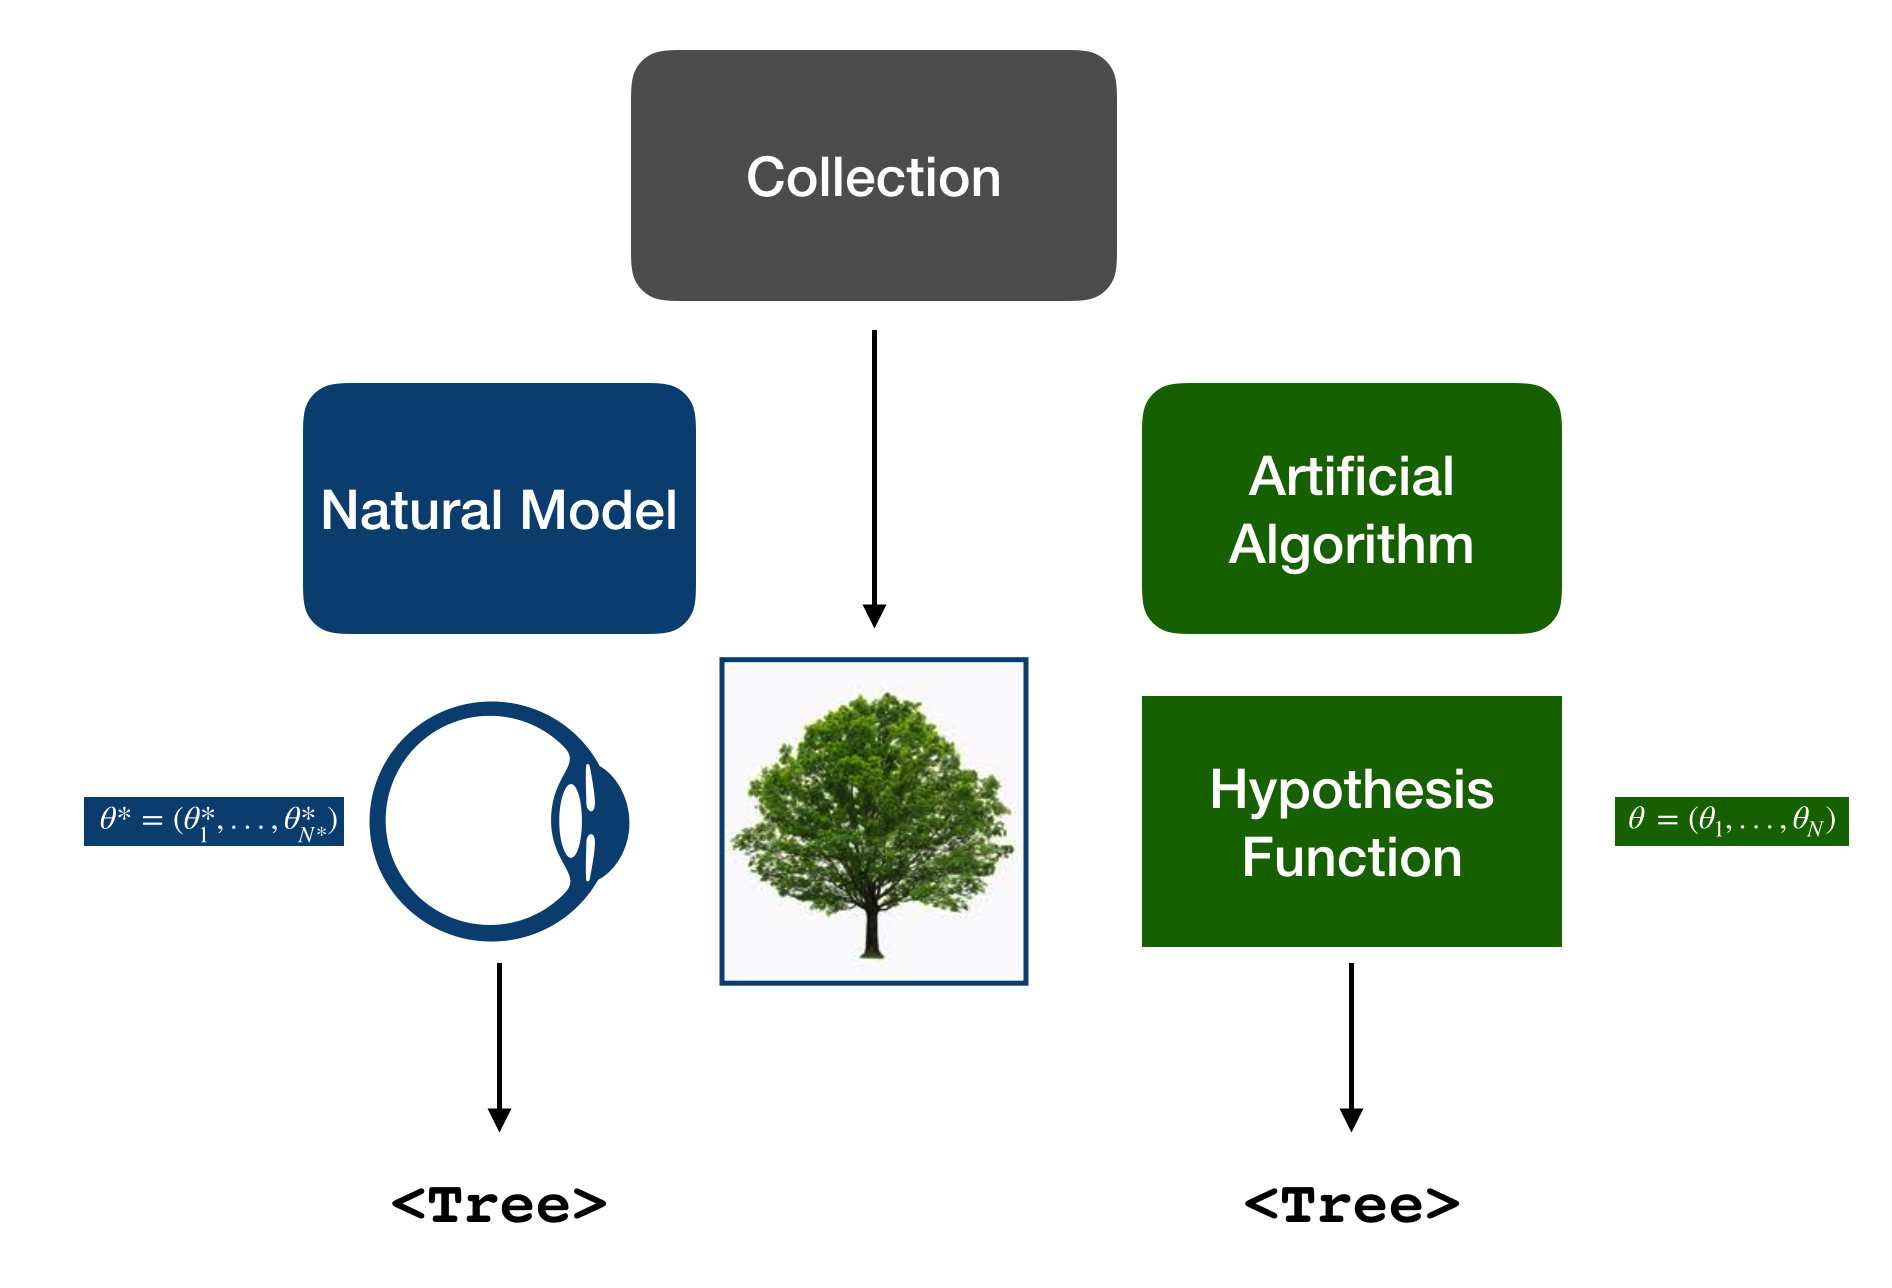
\includegraphics[scale=0.25]{Pics/learning-algorithm.png}
		\end{figure}
	
	\end{frame}

	\begin{frame}{Data Distribution}
		\begin{itemize}
			\item \alert{\textbf{Assumption:}} Data points are arrived i.i.d from a random distribution.\begin{itemize}
				\item A random point generator with some parameters.
				\item Entities are points in $\R^d$. \pause
				\item Data entity $\langle x^{(i)},y^{(i)} \rangle$ has $y^{(i)} = c$ for some constant $c$, and $x^{(i)} = [x^{(i)}_1 , ... , x^{(i)}_d]$ for some fixed $d$ over all $i$s.
			\end{itemize}\pause
			\item \textbf{Sequential Data:} Each data entity $\langle x^{(i)},y^{(i)} \rangle$ has $y^{(i)} = [y^{(i), 1} , ... , y^{(i), T_i}]$ and $x^{(i)} = [x^{(i), 1} , ... , x^{(i), T_i}]$ in which, each of $x^{(i) , j}$ could be it self a vector of fixed length $d$.
		\end{itemize}
	
	\end{frame}

	\begin{frame}{ML Usual Procedure}
		\begin{figure}
			\centering
			\caption{Supervised Learning Procedure}
			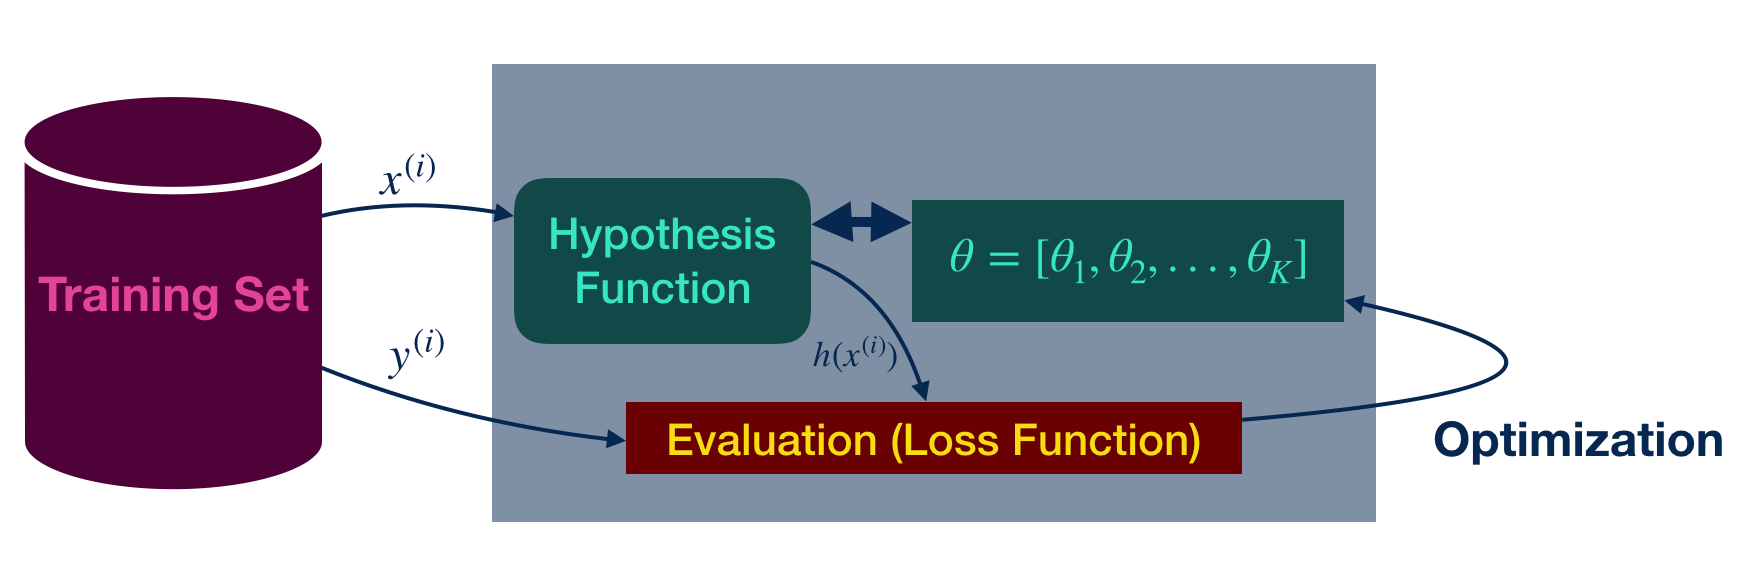
\includegraphics[scale=0.4]{Pics/supervised-learning.png}
		\end{figure}
	\end{frame}

\section{Sequence Data}
	\begin{frame}{Sequence Data}
		\begin{columns}
			\begin{column}{0.6\textwidth}
				\begin{itemize}
					\item<1-> Time Series Data\begin{itemize}
						\item \textbf{Discrete:} Values of currency exchange.
						\item \textbf{Continues:} Speech signal, Video data.
					\end{itemize}
					\item<2-> Other Series:\begin{itemize}
						\item DNA and Gene data
						\item Sentence data
					\end{itemize}
				\end{itemize}
			\begin{itemize}
				\item <3-> Sequential Stationary Distribution \\ \tiny Data evolves but distribution is stationary. \normalsize
				\item <4-> Sequential Un-stationary Distribution \\ \tiny Distribution evolves.
			\end{itemize}
			\end{column}
			\begin{column}{0.4\textwidth}
				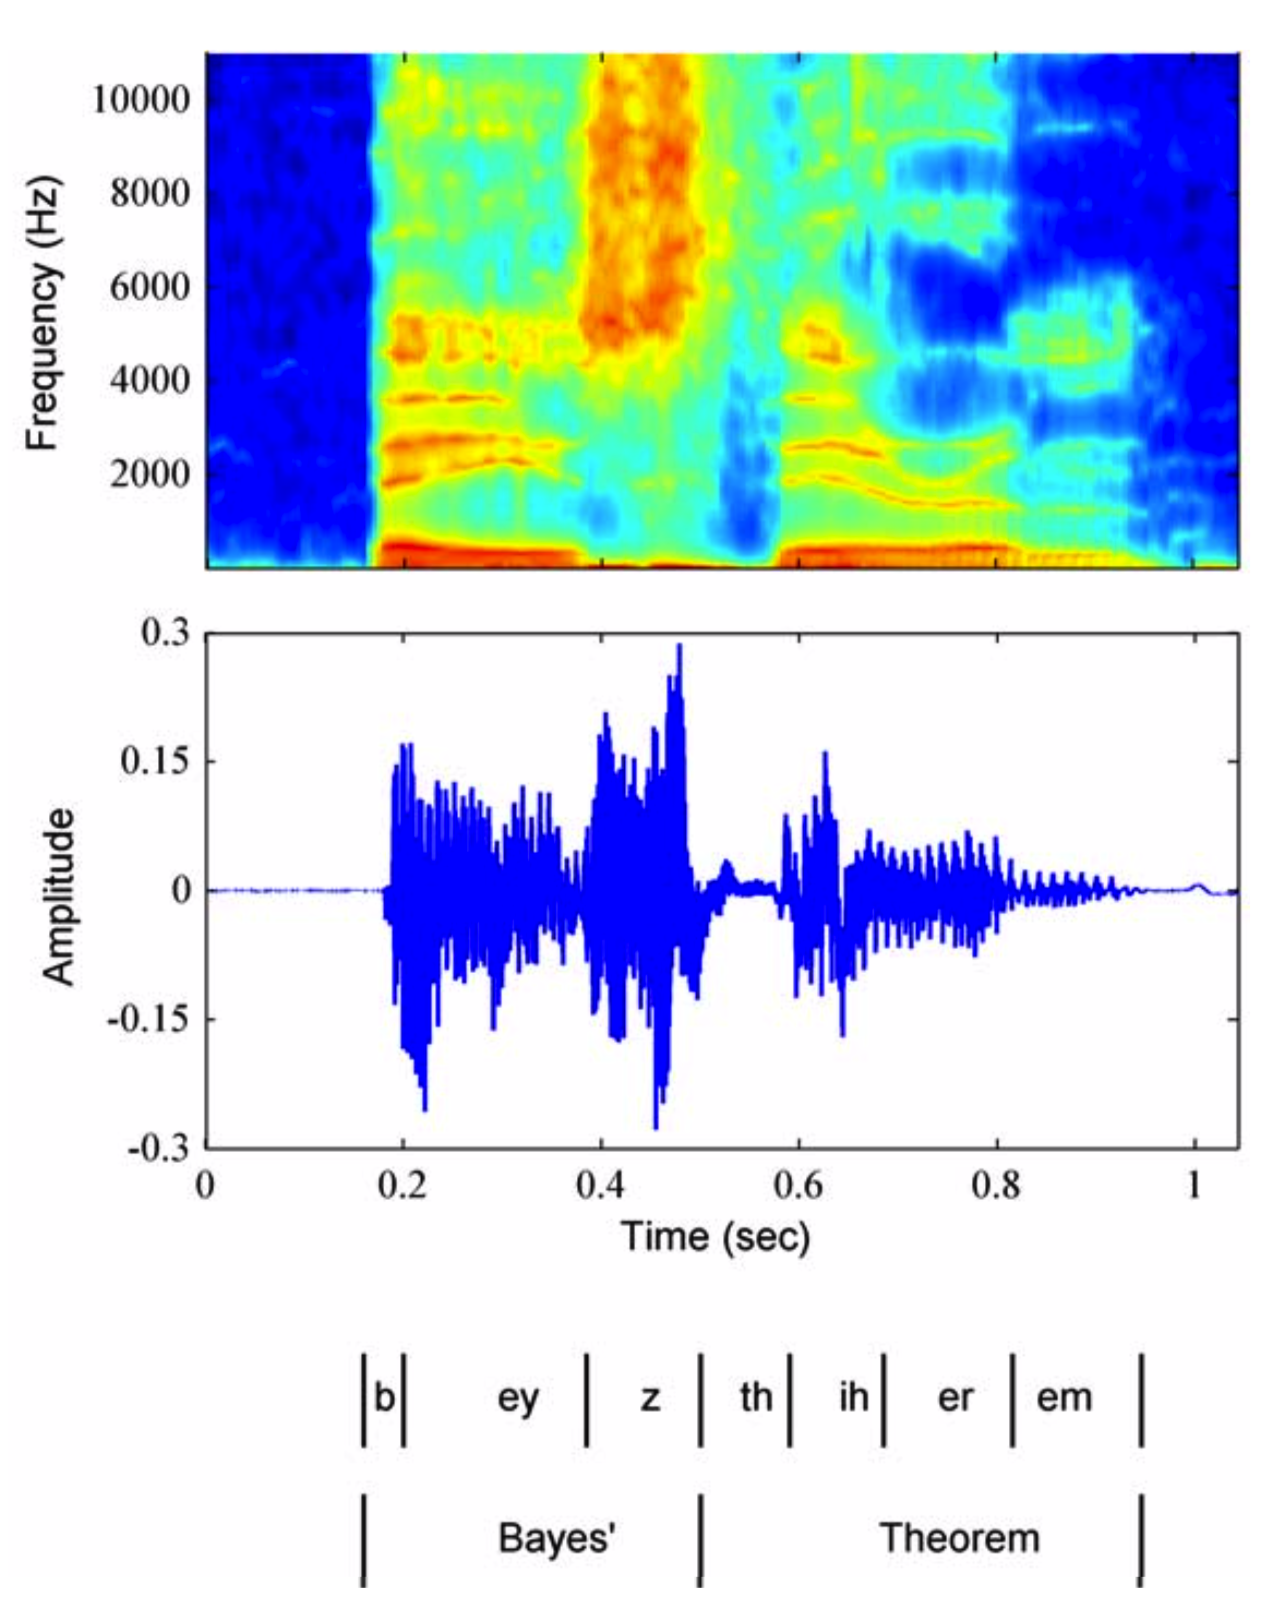
\includegraphics[scale=0.2]{pics/sequencedata.png}
			\end{column}
		\end{columns}
	\end{frame}

	\begin{frame}{Two Different Problems}
		\begin{columns}
			\begin{column}{0.5\textwidth}
				\begin{center}
					\textbf{Sequential Supervised\\ Learning}
					\begin{itemize}
						\item<1-> The entire input in all timestamps is given before we make any predictions.
						\item<2-> The task is to estimate all $[y^1 , ... , y^T]$.
						\item<3-> We don't have access to $y$ values at any time. We should do the prediction on all $y$s at once.
						
					\end{itemize}
				\end{center}
			\end{column}
			\begin{column}{0.5\textwidth}
				\begin{center}
					\textbf{Time-Series\\ Prediction}
					\begin{itemize}
						\item<1-> We have only the prefix of data entity until the current time-stamp.
						\item<2-> The task is to find predict $t+1$-st element of $y$. 
						\item<3-> We have access to the true value of $[y^1 , ... , y^T]$ when predicting $y^{T + 1}$
					\end{itemize}
				\end{center}
			\end{column}
		\end{columns}
	\end{frame}

	\begin{frame}{Third Problem: Sequence Classification}
		Problem statement is that given a sequence data, determine a single label value according to the whole observation. \begin{itemize}
			\item Given data is in form  $\{ \langle x^{(i)},y^{(i)} \rangle_{i = 1}^{N} \}$ where $x^{(i)}$ is a sequence $x^{(i)} = [x^{(i) , 1} , ... , x^{(i), T_i}]$
			\begin{itemize}
				\item Handwritten recognition
				\item Speaker identification
				\item Emotion Recognition
			\end{itemize}
		\end{itemize}
	\end{frame}

\section{General Models}
	\begin{frame}{Ways to Treat Sequential Data}
		\begin{itemize}
			\item<1-> Disrespect the sequential properties of data and treat each time-stamp independent. \begin{itemize}
				\item<2-> Each frame does not contain enough information.
				\item<3-> Fail to exploit the sequential patterns.
				
			\item<4-> Without lose of generality we can express a joint distribution that \[ p(x_1 , ... , x_N)  = \prod_{n = 1}^{N}p(x_n \mid x_{n - 1},...,x_1) \] 
			
			\end{itemize}
		\item<5-> Treat sample with respect to $k$ (or $k(t)$) previous observation.
		\item<6-> Find some patterns in samples and use them to classify with non-sequential data techniques.
		\item<7-> Use embedding.
		\end{itemize}
	\end{frame}

	\begin{frame}{Markov Models}
		Assuming that $ p(x_1 , ... , x_N)  = \prod_{n = 1}^{N}p(x_n \mid x_{n - 1},...,x_1) $:
		\begin{figure}\centering \includegraphics[scale=0.2]{iid.png}
			\includegraphics[scale=0.2]{firstorder.png}\end{figure} 
		\begin{itemize} 
			\item Assuming that any sample is derived i.i.d from a distribution. \[ p(x_n\mid x_{n - 1},...,x_1) = p(x_n) \] \pause
			\item First Order Markov model \[ p(x_n\mid x_{n - 1},..., x_{1}) = p(x_n\mid x_{n - 1}) \] which results $p(x_1, ... , x_n) = p(x_1)\prod_{i = 2}^{n}p(x_i \mid x_{i - 1})$ 
		\end{itemize}
	\end{frame}

	\begin{frame}{Markov Models}
		\begin{definition}[$k$-th Order Markov Chain]
			Assuming that \[ p(x_n\mid x_{n-1}, ... , x_1) = p(x_n\mid x_{n - 1}, x_{n - 2}, x_{n - 3}) \] which implies \[ p(x_1 , ... , x_N) = \prod_{i = 1}^{k} p(x_i \mid x_1 , ... , x_{i - 1}) \times \prod_{n = k+1}^{N} p(x_n\mid x_{n - 1},...,x_{n - k}) \]
		\end{definition}
	\pause
		\alert{Drawbacks:} \begin{itemize}
			\item For large $k$s its not efficient. 
			\item Again it is restricted to certain previous frames.
		\end{itemize} 
	\end{frame}	
	

	\begin{frame}{Formal Definition: Markov Chain}
		A random process over finite alphabet $[k] = \{ 1 , 2 , ... , k \}$;
		\begin{itemize}
			\item Considered to be i.i.d. by defining a single distribution $p$ over $[k]$. The only requirement is a function having Kolmogorov properties.
			\item \textbf{Markov Chain} is defined by a transition probability matrix $M$ over $[k]\times [k]$, and an initial probability $\mu$. 
		\end{itemize}\pause
		Given a sequence of observations $X^n = (x_1 , ... , x_n)$ we seek to find a transition matrix $M:[k]\times[k]\rightarrow \R$ which minimizes the loss function \[ \rho_n^L(P , P') = \E_{X^n \sim P} [L(P_{X^n}, P'_{X^n})] \]
	\end{frame}



	\begin{frame}{Formal Definition: Markov Chain}
		Also can be described as graph, in which each edge has a weight corresponding to the probability of moving from one end point to the other. \pause As a result, 
		
		\begin{theorem}
			Let $P$ be the transition matrix of a Markov chain, the $ij$th entry of $P^{n}$ denotes the probability of reaching $s_j$ n steps after being in $s_i$.
		\end{theorem} \pause
	
			\begin{itemize}
			\item Probability of a sequence $X = (x_1 , ... , x_n)$ be generated by Markov chain $(M , \mu)$ is \[
			P = (\mu(x_1))\times \prod_{i = 2}^{n}M(x_i , x_{i - 1})
			\]
		\end{itemize}
	\end{frame}


	\begin{frame}
		\alert{\textbf{Problem: }}Given numbers of corpus of text (or other sequence), the query is that to what corpus does the given sentence belong. (Find how far a sentence is from the context of each corpus.) \pause Example:
		\begin{columns}
			\begin{column}{0.5\textwidth}
					\begin{tcolorbox}[colback=GrL,colframe=CD,title=The Phantom of the Opera]
					\tiny The Opera ghost really existed. He was not, as was long believed,
					a creature of the imagination of the artists, the superstition of
					the managers, or a product of the absurd and impressionable brains
					of the young ladies of the ballet, their mothers, the box-keepers,
					the cloak-room attendants or the concierge. Yes, he existed
					in flesh and blood, although he assumed the complete appearance
					of a real phantom; that is to say, of a spectral shade.
					
					When I began to ransack the archives of the National Academy of
					Music   ...
				\end{tcolorbox}
			\end{column}
			\begin{column}{0.5\textwidth}
				\begin{tcolorbox}[colback=GrL,colframe=CD,title=Sherlock Holmes]
					\tiny To Sherlock Holmes she is always the woman. I have seldom heard him
					mention her under any other name. In his eyes she eclipses and
					predominates the whole of her sex. It was not that he felt any
					emotion akin to love for Irene Adler. All emotions, and that one
					particularly, were abhorrent to his cold, precise but admirably
					balanced mind. He was, I take it, the most perfect reasoning and
					observing machine that the world has seen, but as a lover he would
					have placed himself in a false position. He never spoke of the softer
					passions, save with a
					...
				\end{tcolorbox}
			\end{column}
			
		\end{columns}\pause
		To which does the sentence
		\begin{tcolorbox}[colback=GrL]
			\tiny For several months, there had been nothing discussed
			at the Opera but this ghost in dress-clothes who stalked about
			the building, from top to bottom, like a shadow, who spoke to nobody,
			to whom nobody dared speak and who vanished as soon as he was seen,
			no one knowing how or where.
		\end{tcolorbox}
		 belongs?
	
	\end{frame}
	\begin{frame}{$N$-gram Model}
		Given a set of observations $X = (x_1 , ... , x_n)$ an $N$-gram model is defined as following \begin{itemize}
			\item<1-> Assign a probability to each possible $p(w_N\mid w_{N - 1}, ..., w_1)$ for each possible tuple $(w_N , w_{N - 1} , ... , w_1)$.
			
			\item<2-> Define an smoothing function in case that the occurrence of  $(w_N , w_{N - 1} , ... , w_1)$ is zero in the corpus. 
			
			\item<3-> Add a start token for the beginning of the sentence. 
		\end{itemize}
	\end{frame}
	\begin{frame}{$N$-gram Model - Perplexity}
		\begin{definition}
			Given that \[
			P_C(S) = \prod_{i = 1}^{|S|} P_C(s_i\mid s_{i - 1},s_{i - 2},..., s_{i - N})
			\]
			The perplexity of a sentence to the corpus is defined as \[
			PPL_C(S) = P_C(S)^{-1/|S|}
			\]
		\end{definition}
		The less the perplexity is due to a corpus the more it is supposed to be derived from that corpus. 
	\end{frame}
	
	\begin{frame}{$N$-gram Points and Drawbacks}
		\begin{itemize}
			\item<1-> It really needs smoothing function. Otherwise in many cases the probability becomes zero.
			\item<2-> Needs a large training corpus. Small training corpus can not result the model to understand the context and semantics.
			\item<3-> It is inefficient both in time and memory. There are $|\Sigma|^N$ possible probabilities. (Check out suffix tree which can reduce the space and time \alert{but not significantly}.)
		\end{itemize}
	\end{frame}

	\begin{frame}{Hidden Markov Model}
		\begin{columns}
			\begin{column}{0.65\textwidth}
				\begin{itemize}
					\item<1-> The model is supposed to be a Markov model with unobservable states. 
					\begin{itemize}
						\item<2-> A set of \textit{latent variables} $q_1 , ... , q_N$ showing the \alert{\textit{hidden states}}.
						\item<2-> States are working same as Markov chain (having \textit{\alert{transition probability}} matrix $A_{N\times N}$).
						\item<3-> A set of \alert{\textit{observations}} $o_1 , ... , o_t$
						\item<3-> Matrix of \alert{\textit{observation likelihood}} or \textit{emotion probability} measuring the probability of that observation $o_t$ is made by state $q_n$. (Matrix $B_{N\times T}$)
						\item<4-> \alert{\textit{Initial probabilities}} $\pi_1 , ... , \pi_N$ over distributions.
					\end{itemize}
				\end{itemize}
			\end{column}
			\begin{column}{0.35\textwidth}
				\begin{center}
					\includegraphics<1>[scale=0.25]{Pics/hmm1.png}
					\includegraphics<2>[scale=0.25]{Pics/hmm2.png}
					\includegraphics<3->[scale=0.25]{Pics/hmm3.png}
					
				\end{center}
			\end{column}
		\end{columns}
		
	\end{frame}

	\begin{frame}{Hidden Markov Model}
		Basic Problems:
		\begin{description}
			\item[Likelihood]<1-> Given the HMM model $\lambda = (A , B)$ and an observation $O$, determine $p(O\mid \lambda)$
			\item[Decoding]<2-> Given the HMM model $\lambda = (A ,B)$ and an observation $O$, find the best state sequence from $[Q]^{|O|}$ that causes the observation.
			\item[Learning]<3-> Given the observation (or observation set) train the HMM model (find best $A$ and $B$).
		\end{description}
	\end{frame}

\section{Sequential Supervised Learning}
	\begin{frame}{Recall; Sequential Supervised Learning}
		\begin{center}
			\textbf{Sequential Supervised Learning}
			\begin{itemize}
				\item The entire input in all timestamps is given before we make any predictions.
				\item The task is to estimate all $[y^1 , ... , y^T]$.
				\item We don't have access to $y$ values at any time. We should do the prediction on all $y$s at once.
			\end{itemize}
		\end{center}
	\end{frame}

	\begin{frame}{Sliding Window Approach}
		It is considered as a way to convert data in order to use classical supervised learning methods. 
		\begin{itemize}
			\item<1-> Assume $w$ to be the window size; assign $d:= (w - 1)/2$. 
			\item<2-> Pad $d$ ``null'' symbols at the beginning and end of the sequence.
			\item<3-> For each $1 \le i \le N$ and $1 \le t \le || x^{(i)}$ create a data entity $x^{(i , t)} := [x^{(i), t - d}, x^{(i), t - d + 1}, ... ,x^{(i), t} , x^{(i), t + 1} , ... , x^{(i), t + d}]$ and $y^{(i , t)} = y^{(i) , t}$
			\item<4-> Using the classical unsupervised training, train the hypothesis function $h_w$ with the new dataset.
			
		\end{itemize}
		\begin{center}
			\includegraphics<1>[scale=0.3]{Pics/revolving-window1.png}
			\includegraphics<2>[scale=0.3]{Pics/revolving-window2.png}
			\includegraphics<3>[scale=0.3]{Pics/revolving-window4.png}
			\includegraphics<4>[scale=0.3]{Pics/revolving-window4.png}
		\end{center}
	\end{frame}
	\begin{frame}{Sliding Window Approach}
		\begin{description}
			\item[Recurrent Sliding Window] Adding the predicted value $\bar{y}_t$ to the next window entity.
		\end{description}
		\begin{center}
			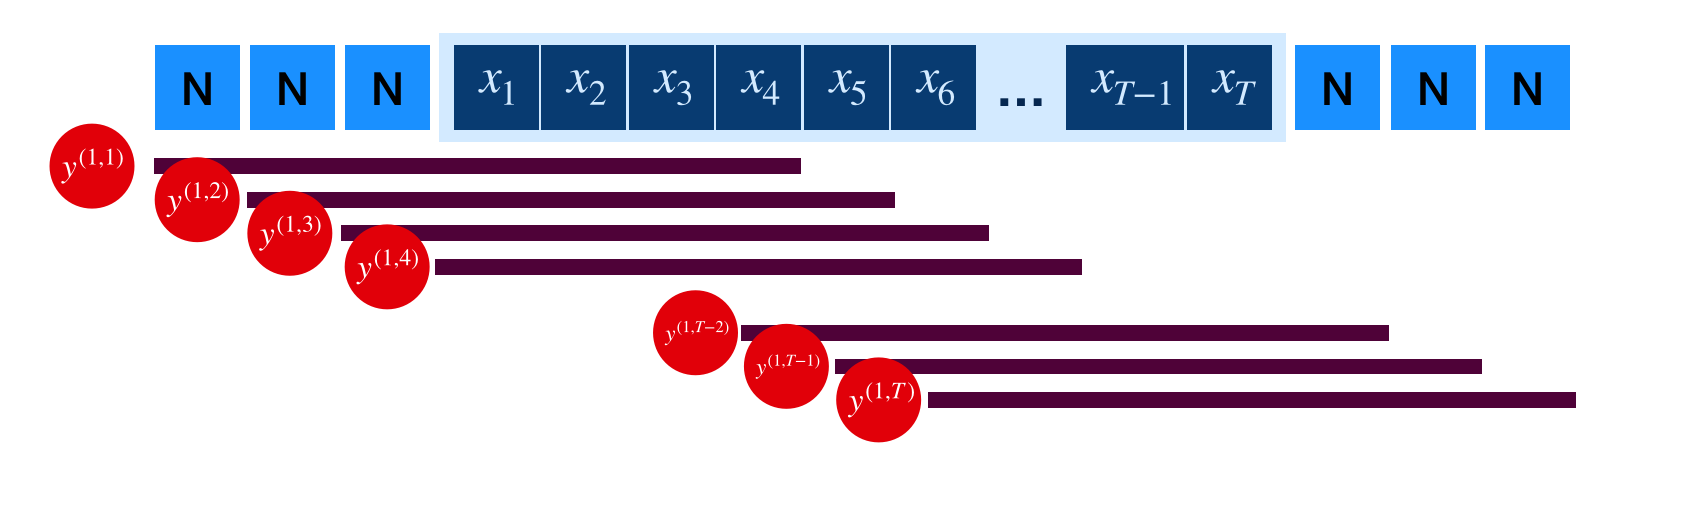
\includegraphics[scale=0.4]{Pics/rec-window.png}
		\end{center}
	\end{frame}

	
%	\begin{frame}{Conditional Random Fields}
%		
%	\end{frame}

\section{Sequence Classification}
	\begin{frame}{Recall; Sequence Classification}
		Problem statement is that given a sequence data, determine a single label value according to the whole observation. \begin{itemize}
			\item Given data is in form  $\{ \langle x^{(i)},y^{(i)} \rangle_{i = 1}^{N} \}$ where $x^{(i)}$ is a sequence $x^{(i)} = [x^{(i) , 1} , ... , x^{(i), T_i}]$.
			
			\pause
			The input data is totally characterized in one below;
			\begin{itemize}[<+->]
				\item Given an alphabet set $\Sigma$, \alert{\textit{simple symbolic sequence}} is an ordered list of symbols. 
				\item A \alert{\textit{complex symbolic sequence}} is an ordered list of vectors each as a subset of alphabets.
				\item A \alert{\textit{simple time series} }is a real value ordered in timestamps.
				\item A \alert{\textit{multivariate time series}} is a series of numerical vectors ordered by timestamps.
				\item A \alert{\textit{complex event sequence}} is the containing the general form in which each event can be a more complex structure such as graph or etc.
			\end{itemize}
		\end{itemize}
	\end{frame}
	
	\begin{frame}{Sequence Classification Methods}
		\begin{center}
			\textbf{Challenges}
		\end{center}
		\begin{itemize}[<+->]
			\item Most of the classification algorithms work with input data as a vector of features, \alert{there are no explicit features in sequence data}.
			\item Even by transforming a sequence to a set of features \alert{the feature selection is far from trivial.}
			\item \alert{Building an interpretable classifier is far from trivial} since no explicit feature exists.
		\end{itemize}
		
	\end{frame}

	\begin{frame}{Sequence Classification Methods}
		\begin{center}
			\textbf{Category of Methods}
		\end{center}
		\begin{itemize}[<+->]
			\item \alert{Feature Based Classification}; transforms a sequence to a feature vector. The next step is to use conventional classification methods.
			\item \alert{Sequence Distance Based Classification}; A distance function is needed to find the similarity of two given sequences. (eg. longest common subsequence)
			\item \alert{Model Based Classification} eg. HMM.
		\end{itemize}
	\end{frame}
	\begin{frame}{Feature Based Classification}
	\alert{Feature Based Classification}; transforms a sequence to a feature vector. The next step is to use conventional classification methods. \pause
		\begin{itemize}
			\item $k$-grams \pause
			\item Choose features as short segments having following conditions;
			\begin{itemize}
				\item Frequent in at least one class
				\item Distinctive in at least one class
				\item Not redundant
			\end{itemize}\pause
			\item \alert{Time series shapelets}. A shapelet is a segment of time series which can be used to separate the training data into two parts according to the distance to the shapelet, and maximizes the information gain.\pause
			\item Modify \alert{wavelet decomposition} to describe a symbolic sequence on multiple resolutions.
		\end{itemize}
	\end{frame}
	\begin{frame}{Sequence-Distance Based Classification}
		Once a distance function is determined, we can use classification algorithms like KNN, SVM with local alignment, spectral kernel representation, etc.
		
		There are some usual distance functions for sequences; 
		\begin{itemize}[<+->]
			\item Euclidean Distance; Requires the sequence to be of same length.
			\item Dynamic Time Warping Distance;
			\item Alignment Based Distances; For DNA sequences, etc.
			
		\end{itemize}
	\end{frame}

	\

	\begin{frame}[plain]
	\begin{center}
		\includegraphics[scale = 0.18]{ramanujan.jpeg}\\
		\textcolor{CD}{\Large{Srinivasa Ramanujan} \\ \rule{\linewidth}{2pt}}\\[5pt]
		\normalsize An equation for me has no meaning, unless it expresses a thought of God.\\ \textcolor{CD}{\rule{\linewidth}{2pt}}
	\end{center}
	\end{frame}


\end{document}